Figure - Improvement in imputation accuracy for the South African population Sotho upon utilization of a merged reference panel.

Figure - Correlation between improvement in imputation accuracy (y-axis) and smallest FST from a 1000G population (x-axis). The FST is calculated between each African population and each of the 1000G populations. The smallest value is plotted on the x-axis. The improvement in imputation accuracy - as measured by change in overall r2 reported by IMPUTE2 when using a 1000G and a 1000G+AGV reference panel - is plotted on the y-axis. Presumably Sotho improves more than any other population, because no South African population is present in 1000G, whereas the AGV reference panel contains a Zulu population. Likewise an infinitesimal improvement is observed for the Igbo population, because the neighboring Yoruba population is already present in 1000G. However, all African populations improve to a higher accuracy upon using the AGV reference panel in combination with 1000G and on its own (data not shown).

\subsection{Correlation and mirror alleles}
We calculated the genotype correlation for all 12 (4*(4-1)) possible heterozygous allele combinations. We found that the alleles with complementary mirror alleles (i.e. AT and CG), which can cause strand ambiguity, have lower overall correlation than other heterzogyous allele types (figure \ref{fig:imp_accu_allele}. Therefore we recommend that whenever possible alleles, which can cause problems in determining the relative strand, are not included on any future chip.

\begin{figure}[htp]
\centering
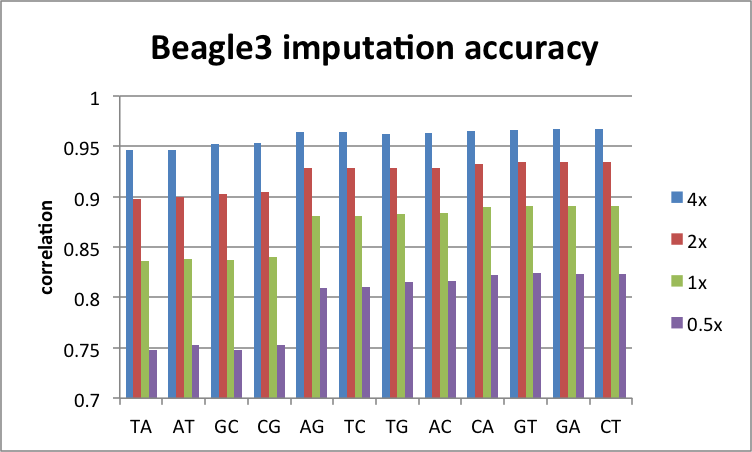
\includegraphics{Chapter3/fig/imp_accu_allele}
\caption{Imputation accuracy for each heterzygous allele. We used the Baganda 4x sequence data and SNP array data to calculate the genotype correlation for each heterozygous allele type. We found that the "mirror" alleles AT/TA and CG/GC for which it can be difficult to determine the relative strand have lower genotype correlations. }
\label{fig:imp_accu_allele}
\end{figure}